% Created 2024-02-27 ti 13:50
% Intended LaTeX compiler: pdflatex
\documentclass[12pt]{article}

%%%% settings when exporting code %%%% 

\usepackage{listings}
\lstdefinestyle{code-small}{
backgroundcolor=\color{white}, % background color for the code block
basicstyle=\ttfamily\small, % font used to display the code
commentstyle=\color[rgb]{0.5,0,0.5}, % color used to display comments in the code
keywordstyle=\color{black}, % color used to highlight certain words in the code
numberstyle=\ttfamily\tiny\color{gray}, % color used to display the line numbers
rulecolor=\color{black}, % color of the frame
stringstyle=\color[rgb]{0,.5,0},  % color used to display strings in the code
breakatwhitespace=false, % sets if automatic breaks should only happen at whitespace
breaklines=true, % sets automatic line breaking
columns=fullflexible,
frame=single, % adds a frame around the code (non,leftline,topline,bottomline,lines,single,shadowbox)
keepspaces=true, % % keeps spaces in text, useful for keeping indentation of code
literate={~}{$\sim$}{1}, % symbol properly display via latex
numbers=none, % where to put the line-numbers; possible values are (none, left, right)
numbersep=10pt, % how far the line-numbers are from the code
showspaces=false,
showstringspaces=false,
stepnumber=1, % the step between two line-numbers. If it's 1, each line will be numbered
tabsize=1,
xleftmargin=0cm,
emph={anova,apply,class,coef,colnames,colNames,colSums,dim,dcast,for,ggplot,head,if,ifelse,is.na,lapply,list.files,library,logLik,melt,plot,require,rowSums,sapply,setcolorder,setkey,str,summary,tapply},
aboveskip = \medskipamount, % define the space above displayed listings.
belowskip = \medskipamount, % define the space above displayed listings.
lineskip = 0pt} % specifies additional space between lines in listings
\lstset{style=code-small}
%%%% packages %%%%%

\usepackage[utf8]{inputenc}
\usepackage[T1]{fontenc}
\usepackage{lmodern}
\usepackage{textcomp}
\usepackage{color}
\usepackage{graphicx}
\usepackage{grffile}
\usepackage{wrapfig}
\usepackage{rotating}
\usepackage{longtable}
\usepackage{multirow}
\usepackage{multicol}
\usepackage{changes}
\usepackage{pdflscape}
\usepackage{geometry}
\usepackage[normalem]{ulem}
\usepackage{amssymb}
\usepackage{amsmath}
\usepackage{amsfonts}
\usepackage{dsfont}
\usepackage{array}
\usepackage{ifthen}
\usepackage{hyperref}
\usepackage{natbib}
%
%%%% specifications %%%%
%
\usepackage{ifthen}
\usepackage{xifthen}
\usepackage{xargs}
\usepackage{xspace}
\RequirePackage{fancyvrb}
\DefineVerbatimEnvironment{verbatim}{Verbatim}{fontsize=\small,formatcom = {\color[rgb]{0.5,0,0}}}
\RequirePackage{colortbl} % arrayrulecolor to mix colors
\RequirePackage{setspace} % to modify the space between lines - incompatible with footnote in beamer
\renewcommand{\baselinestretch}{1.1}
\geometry{top=1cm}
\RequirePackage{colortbl} % arrayrulecolor to mix colors
\RequirePackage{pifont}
\RequirePackage{relsize}
\newcommand{\Cross}{{\raisebox{-0.5ex}%
{\relsize{1.5}\ding{56}}}\hspace{1pt} }
\newcommand{\Valid}{{\raisebox{-0.5ex}%
{\relsize{1.5}\ding{52}}}\hspace{1pt} }
\newcommand{\CrossR}{ \textcolor{red}{\Cross} }
\newcommand{\ValidV}{ \textcolor{green}{\Valid} }
\usepackage{stackengine}
\usepackage{scalerel}
\newcommand\Warning[1][3ex]{%
\renewcommand\stacktype{L}%
\scaleto{\stackon[1.3pt]{\color{red}$\triangle$}{\tiny\bfseries !}}{#1}%
\xspace
}
\hypersetup{
citecolor=[rgb]{0,0.5,0},
urlcolor=[rgb]{0,0,0.5},
linkcolor=[rgb]{0,0,0.5},
}
\RequirePackage{epstopdf} % to be able to convert .eps to .pdf image files
\RequirePackage{capt-of} %
\RequirePackage{caption} % newlines in graphics
\RequirePackage{tikz}
\definecolor{grayR}{HTML}{8A8990}
\definecolor{grayL}{HTML}{C4C7C9}
\definecolor{blueM}{HTML}{1F63B5}
\newcommand{\Rlogo}[1][0.07]{
\begin{tikzpicture}[scale=#1]
\shade [right color=grayR,left color=grayL,shading angle=60]
(-3.55,0.3) .. controls (-3.55,1.75)
and (-1.9,2.7) .. (0,2.7) .. controls (2.05,2.7)
and (3.5,1.6) .. (3.5,0.3) .. controls (3.5,-1.2)
and (1.55,-2) .. (0,-2) .. controls (-2.3,-2)
and (-3.55,-0.75) .. cycle;

\fill[white]
(-2.15,0.2) .. controls (-2.15,1.2)
and (-0.7,1.8) .. (0.5,1.8) .. controls (2.2,1.8)
and (3.1,1.2) .. (3.1,0.2) .. controls (3.1,-0.75)
and (2.4,-1.45) .. (0.5,-1.45) .. controls (-1.1,-1.45)
and (-2.15,-0.7) .. cycle;

\fill[blueM]
(1.75,1.25) -- (-0.65,1.25) -- (-0.65,-2.75) -- (0.55,-2.75) -- (0.55,-1.15) --
(0.95,-1.15)  .. controls (1.15,-1.15)
and (1.5,-1.9) .. (1.9,-2.75) -- (3.25,-2.75)  .. controls (2.2,-1)
and (2.5,-1.2) .. (1.8,-0.95) .. controls (2.6,-0.9)
and (2.85,-0.35) .. (2.85,0.2) .. controls (2.85,0.7)
and (2.5,1.2) .. cycle;

\fill[white]  (1.4,0.4) -- (0.55,0.4) -- (0.55,-0.3) -- (1.4,-0.3).. controls (1.75,-0.3)
and (1.75,0.4) .. cycle;

\end{tikzpicture}
}
\RequirePackage{enumitem} % to be able to convert .eps to .pdf image files
\definecolor{light}{rgb}{1, 1, 0.9}
\definecolor{lightred}{rgb}{1.0, 0.7, 0.7}
\definecolor{lightblue}{rgb}{0.0, 0.8, 0.8}
\newcommand{\darkblue}{blue!80!black}
\newcommand{\darkgreen}{green!50!black}
\newcommand{\darkred}{red!50!black}
\usepackage{mdframed}
\newcommand{\first}{1\textsuperscript{st} }
\newcommand{\second}{2\textsuperscript{nd} }
\newcommand{\third}{3\textsuperscript{rd} }
\RequirePackage{amsmath}
\RequirePackage{algorithm}
\RequirePackage[noend]{algpseudocode}
\RequirePackage{dsfont}
\RequirePackage{amsmath,stmaryrd,graphicx}
\RequirePackage{prodint} % product integral symbol (\PRODI)
\newcommand\defOperator[7]{%
\ifthenelse{\isempty{#2}}{
\ifthenelse{\isempty{#1}}{#7{#3}#4}{#7{#3}#4 \left#5 #1 \right#6}
}{
\ifthenelse{\isempty{#1}}{#7{#3}#4_{#2}}{#7{#3}#4_{#1}\left#5 #2 \right#6}
}
}
\newcommand\defUOperator[5]{%
\ifthenelse{\isempty{#1}}{
#5\left#3 #2 \right#4
}{
\ifthenelse{\isempty{#2}}{\underset{#1}{\operatornamewithlimits{#5}}}{
\underset{#1}{\operatornamewithlimits{#5}}\left#3 #2 \right#4}
}
}
\newcommand{\defBoldVar}[2]{
\ifthenelse{\equal{#2}{T}}{\boldsymbol{#1}}{\mathbf{#1}}
}
\newcommandx\Cov[2][1=,2=]{\defOperator{#1}{#2}{C}{ov}{\lbrack}{\rbrack}{\mathbb}}
\newcommandx\Esp[2][1=,2=]{\defOperator{#1}{#2}{E}{}{\lbrack}{\rbrack}{\mathbb}}
\newcommandx\Prob[2][1=,2=]{\defOperator{#1}{#2}{P}{}{\lbrack}{\rbrack}{\mathbb}}
\newcommandx\Qrob[2][1=,2=]{\defOperator{#1}{#2}{Q}{}{\lbrack}{\rbrack}{\mathbb}}
\newcommandx\Var[2][1=,2=]{\defOperator{#1}{#2}{V}{ar}{\lbrack}{\rbrack}{\mathbb}}
\newcommandx\Binom[2][1=,2=]{\defOperator{#1}{#2}{B}{}{(}{)}{\mathcal}}
\newcommandx\Gaus[2][1=,2=]{\defOperator{#1}{#2}{N}{}{(}{)}{\mathcal}}
\newcommandx\Wishart[2][1=,2=]{\defOperator{#1}{#2}{W}{ishart}{(}{)}{\mathcal}}
\newcommandx\Likelihood[2][1=,2=]{\defOperator{#1}{#2}{L}{}{(}{)}{\mathcal}}
\newcommandx\Information[2][1=,2=]{\defOperator{#1}{#2}{I}{}{(}{)}{\mathcal}}
\newcommandx\Score[2][1=,2=]{\defOperator{#1}{#2}{S}{}{(}{)}{\mathcal}}
\newcommandx\Vois[2][1=,2=]{\defOperator{#1}{#2}{V}{}{(}{)}{\mathcal}}
\newcommandx\IF[2][1=,2=]{\defOperator{#1}{#2}{IF}{}{(}{)}{\mathcal}}
\newcommandx\Ind[1][1=]{\defOperator{}{#1}{1}{}{(}{)}{\mathds}}
\newcommandx\Max[2][1=,2=]{\defUOperator{#1}{#2}{(}{)}{min}}
\newcommandx\Min[2][1=,2=]{\defUOperator{#1}{#2}{(}{)}{max}}
\newcommandx\argMax[2][1=,2=]{\defUOperator{#1}{#2}{(}{)}{argmax}}
\newcommandx\argMin[2][1=,2=]{\defUOperator{#1}{#2}{(}{)}{argmin}}
\newcommandx\cvD[2][1=D,2=n \rightarrow \infty]{\xrightarrow[#2]{#1}}
\newcommandx\Hypothesis[2][1=,2=]{
\ifthenelse{\isempty{#1}}{
\mathcal{H}
}{
\ifthenelse{\isempty{#2}}{
\mathcal{H}_{#1}
}{
\mathcal{H}^{(#2)}_{#1}
}
}
}
\newcommandx\dpartial[4][1=,2=,3=,4=\partial]{
\ifthenelse{\isempty{#3}}{
\frac{#4 #1}{#4 #2}
}{
\left.\frac{#4 #1}{#4 #2}\right\rvert_{#3}
}
}
\newcommandx\dTpartial[3][1=,2=,3=]{\dpartial[#1][#2][#3][d]}
\newcommandx\ddpartial[3][1=,2=,3=]{
\ifthenelse{\isempty{#3}}{
\frac{\partial^{2} #1}{\partial #2^2}
}{
\frac{\partial^2 #1}{\partial #2\partial #3}
}
}
\newcommand\Real{\mathbb{R}}
\newcommand\Rational{\mathbb{Q}}
\newcommand\Natural{\mathbb{N}}
\newcommand\trans[1]{{#1}^\intercal}%\newcommand\trans[1]{{\vphantom{#1}}^\top{#1}}
\newcommand{\independent}{\mathrel{\text{\scalebox{1.5}{$\perp\mkern-10mu\perp$}}}}
\newcommand\half{\frac{1}{2}}
\newcommand\normMax[1]{\left|\left|#1\right|\right|_{max}}
\newcommand\normTwo[1]{\left|\left|#1\right|\right|_{2}}
\date{\today}
\title{Single group analysis with repeated measurements}
\hypersetup{
 colorlinks=true,
 pdfauthor={},
 pdftitle={Single group analysis with repeated measurements},
 pdfkeywords={},
 pdfsubject={},
 pdfcreator={Emacs 27.2 (Org mode 9.5.2)},
 pdflang={English}
 }
\begin{document}

\maketitle
Load packages
\lstset{language=r,label= ,caption= ,captionpos=b,numbers=none}
\begin{lstlisting}
library(LMMstar)
library(lme4)
library(lmerTest)
library(ggplot2)
\end{lstlisting}

Load data and add 'artificial' sex variable and remove some variables:
\lstset{language=r,label= ,caption= ,captionpos=b,numbers=none}
\begin{lstlisting}
data(gastricbypassW)
gastricbypassW$weight2 <- NULL
gastricbypassW$weight3 <- NULL
gastricbypassW$weight4 <- NULL
gastricbypassW$male <- as.numeric(gastricbypassW$id) %% 2
head(gastricbypassW)
\end{lstlisting}

\begin{verbatim}
  id weight1 glucagonAUC1 glucagonAUC2 glucagonAUC3 glucagonAUC4 male
1  1   127.2      5032.50       4942.5      20421.0      9249.45    1
2  2   165.2     12142.50      14083.5      10945.5      7612.50    0
3  3   109.7     10321.35       6202.5      20121.0     17704.50    1
4  4   146.2      6693.00       6631.5      13090.5      4551.00    0
5  5   113.1      7090.50           NA      19155.0     12345.00    1
6  6   158.8     10386.00       7609.5      11778.0      8014.80    0
\end{verbatim}


Reshape data to long format:
\lstset{language=r,label= ,caption= ,captionpos=b,numbers=none}
\begin{lstlisting}
library(reshape2)
gastricbypassL <- melt(gastricbypassW,
                       id.vars = c("id","male","weight1"),
                       measure.var = paste0("glucagonAUC",1:4),
                       variable.name = "time", value.name = "glucagonAUC")
gastricbypassL$time <- gsub("glucagonAUC","",gastricbypassL$time)
gastricbypassL <- gastricbypassL[order(gastricbypassL$id),]
head(gastricbypassL)
\end{lstlisting}

\begin{verbatim}
   id male weight1 time glucagonAUC
1   1    1   127.2    1     5032.50
21  1    1   127.2    2     4942.50
41  1    1   127.2    3    20421.00
61  1    1   127.2    4     9249.45
2   2    0   165.2    1    12142.50
22  2    0   165.2    2    14083.50
\end{verbatim}


\lstset{language=r,label= ,caption= ,captionpos=b,numbers=none}
\begin{lstlisting}
ggSpa <- ggplot(gastricbypassL, aes(x=time, y=glucagonAUC, group=id))
ggSpa <- ggSpa + geom_point() + geom_line()
ggSpa
\end{lstlisting}

\begin{center}
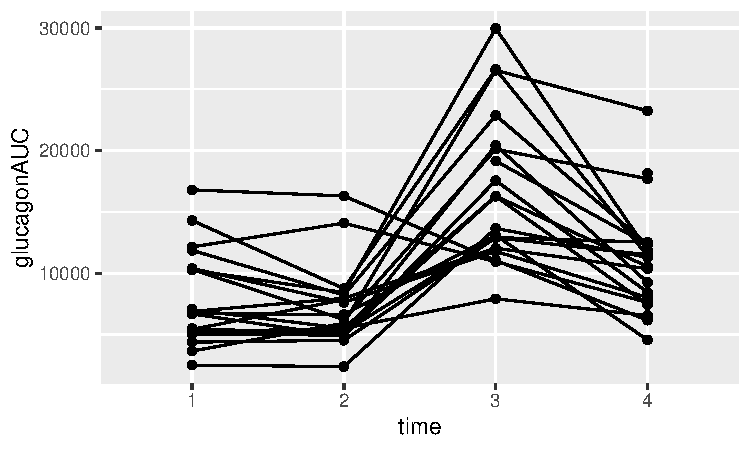
\includegraphics[trim={0 0 0 0},width=1\textwidth]{./figures/gg-spaghettiplot.pdf}
\end{center}

\clearpage

\section{My favorite approach}
\label{sec:org5c04546}

\lstset{language=r,label= ,caption= ,captionpos=b,numbers=none}
\begin{lstlisting}
eUN.lmm <- lmm(glucagonAUC ~ time + male + weight1,
         repetition = ~time | id, structure = "CS",
               data = gastricbypassL)
anova(eUN.lmm) 
\end{lstlisting}

\begin{verbatim}
	     Multivariate Wald test 

              F-statistic       df p.value    
mean: time         14.752 (3,18.0) 4.3e-05 ***
    : male          0.055 (1,11.6)   0.819    
    : weight1       1.308 (1, 7.7)   0.287
\end{verbatim}


\lstset{language=r,label= ,caption= ,captionpos=b,numbers=none}
\begin{lstlisting}
eUN.lmmPairwiseTest <- anova(eUN.lmm,
                effect = c("time2=0","time4=0","time4-time3=0"),
                           multivariate = FALSE)
summary(eUN.lmmPairwiseTest)
\end{lstlisting}

\begin{verbatim}
		Univariate Wald test 

                 estimate       se   df     lower     upper p.value    
   time2         -749.334  485.886 18.9 -2014.107   515.439 0.33716    
   time4         3202.583 1463.277   19  -606.366  7011.531 0.11308    
   time4 - time3 -6007.57  1157.98 16.9 -9021.821 -2993.319 0.00021 ***
   ------------------------------------------------------------------- 
  Signif. codes:  0 '***' 0.001 '**' 0.01 '*' 0.05 '.' 0.1 ' ' 1.
  Columns lower/upper/p.value adjusted for multiple comparisons -- max-test.
  (1e+05 samples have been used)
  Model-based standard errors are derived from the observed information (column se). 
  Degrees of freedom were computed using a Satterthwaite approximation (column df).
\end{verbatim}

\clearpage

\section{Other approach: repeated measurement anova}
\label{sec:orgfeb7cfa}

\lstset{language=r,label= ,caption= ,captionpos=b,numbers=none}
\begin{lstlisting}
e.ranova <- aov(formula = glucagonAUC ~ male + weight1 + time + Error(id),
                 data = gastricbypassL)
summary(e.ranova)
\end{lstlisting}

\begin{verbatim}

Error: id
          Df    Sum Sq   Mean Sq F value Pr(>F)  
male       1   1894331   1894331   0.065 0.8029  
weight1    1 115763362 115763362   3.943 0.0657 .
time       2   7936921   3968460   0.135 0.8746  
Residuals 15 440438932  29362595                 
---
Signif. codes:  0 '***' 0.001 '**' 0.01 '*' 0.05 '.' 0.1 ' ' 1

Error: Within
          Df    Sum Sq   Mean Sq F value   Pr(>F)    
time       3 1.145e+09 381688003   21.77 2.02e-09 ***
Residuals 55 9.645e+08  17537102                     
---
Signif. codes:  0 '***' 0.001 '**' 0.01 '*' 0.05 '.' 0.1 ' ' 1
\end{verbatim}


\clearpage

\section{Other approach: random intercept model}
\label{sec:org15e3612}
\lstset{language=r,label= ,caption= ,captionpos=b,numbers=none}
\begin{lstlisting}
e.lmer <- lmer(glucagonAUC ~ time + male + weight1 + (1 | id),
              data = gastricbypassL)
anova(e.lmer)
\end{lstlisting}

\begin{verbatim}
Type III Analysis of Variance Table with Satterthwaite's method
            Sum Sq   Mean Sq NumDF  DenDF F value    Pr(>F)    
time    1148372460 382790820     3 56.107 21.9527 1.565e-09 ***
male        802158    802158     1 17.281  0.0460   0.83268    
weight1   77654552  77654552     1 17.045  4.4534   0.04991 *  
---
Signif. codes:  0 '***' 0.001 '**' 0.01 '*' 0.05 '.' 0.1 ' ' 1
\end{verbatim}


Same as:
\lstset{language=r,label= ,caption= ,captionpos=b,numbers=none}
\begin{lstlisting}
eCS.lmm <- lmm(glucagonAUC ~ time + male + weight1,
               repetition = ~time | id, structure = "CS",
               data = gastricbypassL)
anova(eCS.lmm) 

\end{lstlisting}

\begin{verbatim}
	     Multivariate Wald test 

              F-statistic       df  p.value    
mean: time          21.95 (3,56.1) 1.57e-09 ***
    : male          0.046 (1,17.3)   0.8327    
    : weight1       4.453 (1,17.1)   0.0499   *
\end{verbatim}
\end{document}